\section{Implementation}
\subsection{Clients}
The three main components are implemented with the low level Java client APIs of the platforms. Consumer clients of the platforms are used to subscribe and read messages on the streams while producer clients are used to publish messages to the platforms.

\begin{figure}[ht!]
	\begin{adjustwidth}{-1cm}{-1cm}
	\centering
	\begin{minipage}[t]{.48\linewidth}
		\centering
		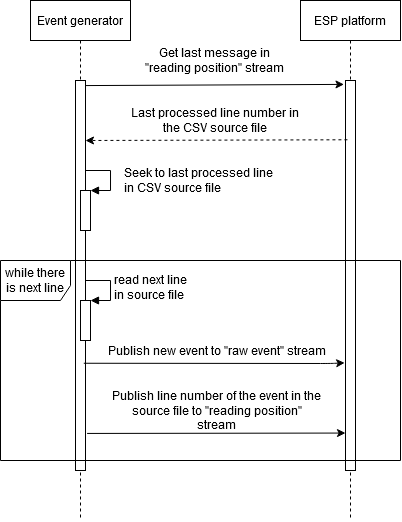
\includegraphics[width=\linewidth]{images/implement-event-generator.png}
		\caption{Sequence diagram of event generator component.}
		\label{fig:implementeventgenerator}
	\end{minipage}%
	\hfill
	\begin{minipage}[t]{.48\linewidth}
		\centering
		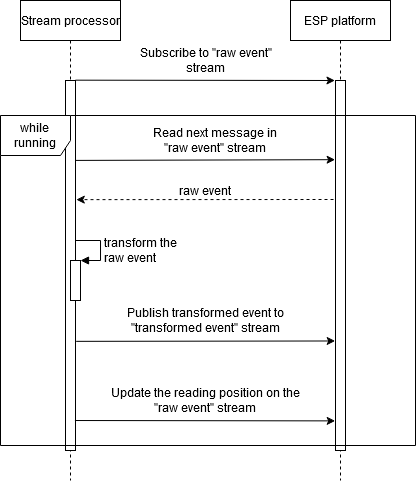
\includegraphics[width=\linewidth]{images/implement-stream-processor.png}
		\caption{Sequence diagram of stream processor component.}
		\label{fig:implementstreamprocessor}
	\end{minipage}
	\end{adjustwidth}
\end{figure}

Figures \ref{fig:implementeventgenerator} and \ref{fig:implementstreamprocessor} show the sequence diagrams of the event generator and the stream processor respectively. With Apache Kafka and Apache Pulsar, to achieve exactly-once semantics with these two components,  the two operations to publish events and update the reading position on the data source must be atomically combined with the transaction features of the two platforms. 

Listing \ref{lst:kafkastreamprocessor} shows part of the source code of the stream processor for Kafka. 

\lstinputlisting[label={lst:kafkastreamprocessor},language=Java,caption={Kafka stream processor with the transaction feature.}]{chapters/implementation/KafkaStreamProcessor.java} 

\lstinputlisting[label={lst:pulsarstreamprocessor},language=Java,caption={Pulsar stream processor with the transaction feature.}]{chapters/implementation/PulsarStreamProcessor.java} 


\subsection{Failure injection}

\subsection{Running environment}
To run the failure scenarios with each platform, Docker compose is used to containerize all components and run them locally in a Docker environment. 